\documentclass[tikz,border=8pt]{standalone}
\usetikzlibrary{arrows.meta, positioning, 3d, calc}

% 3D tensor block: width=channels, height=spatial, depth=time
\newcommand{\tensorblock}[7]{%
  % #1=x, #2=y, #3=width, #4=height, #5=depth, #6=fill color, #7=label
  \begin{scope}[shift={(#1,#2)}]
    % Front face
    \fill[#6!30] (0,0) rectangle (#3,#4);
    \draw[#6!60!black, thick] (0,0) rectangle (#3,#4);
    % Top face (depth)
    \fill[#6!50] (0,#4) -- ++(0.3*#5, 0.3*#5) -- ++(#3,0) -- ++(0,0) -- ++(-0.3*#5,-0.3*#5) -- cycle;
    \draw[#6!60!black, thick] (0,#4) -- ++(0.3*#5, 0.3*#5) -- ++(#3,0) -- ++(-0.3*#5,-0.3*#5) -- cycle;
    % Right face (depth)
    \fill[#6!20] (#3,0) -- ++(0.3*#5,0.3*#5) -- ++(0,#4) -- ++(-0.3*#5,-0.3*#5) -- cycle;
    \draw[#6!60!black, thick] (#3,0) -- ++(0.3*#5,0.3*#5) -- ++(0,#4) -- ++(-0.3*#5,-0.3*#5) -- cycle;
    % Label below
    \node[below, font=\small\sffamily] at (#3/2, -0.15) {#7};
  \end{scope}
}

\begin{document}
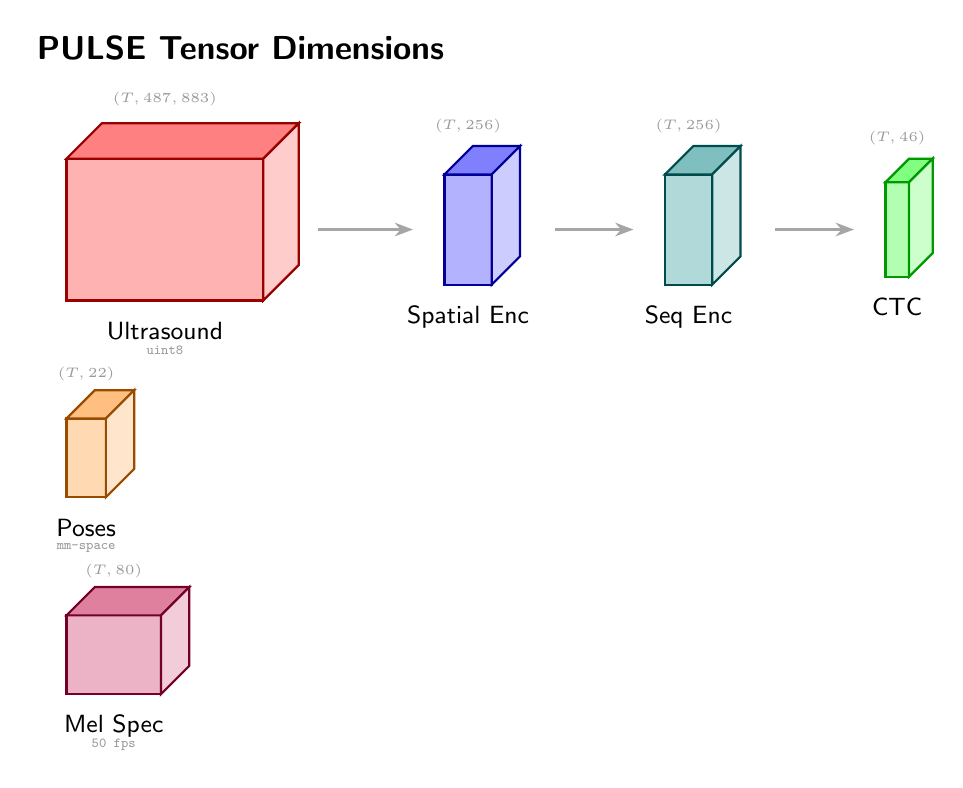
\begin{tikzpicture}[
  arr/.style={-Stealth, thick, gray!70},
  dimlabel/.style={font=\tiny\sffamily, gray!80},
]

% Raw ultrasound: (T, 487, 883) — large block
\tensorblock{0}{0}{2.5}{1.8}{1.5}{red}{Ultrasound}
\node[dimlabel, above] at (1.25, 2.35) {$(T, 487, 883)$};
\node[dimlabel, below=0.3cm] at (1.25, -0.15) {\texttt{uint8}};

% Arrow
\draw[arr] (3.2, 0.9) -- ++(1.2, 0);

% Spatial encoder output: (T, 256) — tall thin block
\tensorblock{4.8}{0.2}{0.6}{1.4}{1.2}{blue}{Spatial Enc}
\node[dimlabel, above] at (5.1, 2.0) {$(T, 256)$};

% Arrow
\draw[arr] (6.2, 0.9) -- ++(1.0, 0);

% Sequence encoder output: (T, 256) — same shape, different color
\tensorblock{7.6}{0.2}{0.6}{1.4}{1.2}{teal}{Seq Enc}
\node[dimlabel, above] at (7.9, 2.0) {$(T, 256)$};

% Arrow
\draw[arr] (9.0, 0.9) -- ++(1.0, 0);

% CTC output: (T, 46) — very thin block
\tensorblock{10.4}{0.3}{0.3}{1.2}{1.0}{green}{CTC}
\node[dimlabel, above] at (10.55, 1.85) {$(T, 46)$};

% Pose input (below, separate branch)
\tensorblock{0}{-2.5}{0.5}{1.0}{1.2}{orange}{Poses}
\node[dimlabel, above] at (0.25, -1.15) {$(T, 22)$};
\node[dimlabel, below=0.3cm] at (0.25, -2.65) {\texttt{mm-space}};

% Mel spectrogram (below poses)
\tensorblock{0}{-5.0}{1.2}{1.0}{1.2}{purple}{Mel Spec}
\node[dimlabel, above] at (0.6, -3.65) {$(T, 80)$};
\node[dimlabel, below=0.3cm] at (0.6, -5.15) {\texttt{50 fps}};

% Title
\node[font=\large\sffamily\bfseries, anchor=west] at (-0.5, 3.2) {PULSE Tensor Dimensions};

\end{tikzpicture}
\end{document}
